% Slide 51: Hyperparameters vs Parameters
\begin{frame}{انتخاب فراپارامترها}{\lr{Hyperparameter Selection}}
  \begin{itemize}
    \setlength{\itemsep}{10pt}
    \item \textbf{فراپارامتر} (\lr{Hyperparameter}): پارامتری است که فرآیند یادگیری الگوریتم را هدایت کرده و مقدار آن \textbf{پیش از آغاز یادگیری} توسط کاربر تعیین می‌شود:
    \begin{itemize}
      \setlength{\itemsep}{3pt}
      \item آستانه هرس در درختان تصمیم (\lr{Pruning Thresholds})
      \item ضرایب $C$ و $\gamma$ در ماشین‌های بردار پشتیبان (\lr{SVM})
      \item نرخ یادگیری (\lr{Learning Rate}) و تعداد لایه‌ها و نورون‌های پنهان در شبکه‌های عصبی
    \end{itemize}
    \item \textbf{پارامترها} (\lr{Parameters}): مقادیری هستند که مستقیماً در طول فرآیند آموزش و از روی داده‌ها یاد گرفته می‌شوند (مانند وزن‌های نورون‌ها $w_i$ یا ضرایب ابرصفحه).
  \end{itemize}
\end{frame}

% Slide 52: Grid Search vs Random Search
\begin{frame}{بهینه‌سازی فراپارامترها}{جستجوی شبکه‌ای در برابر جستجوی تصادفی}
  \begin{columns}[T]
    \begin{column}{0.58\textwidth}
      \begin{itemize}
        \setlength{\itemsep}{2pt}
        \item \textbf{هدف:} یافتن ترکیبی از فراپارامترها با کمترین خطای تعمیم مدل.
        \item \textbf{روش‌های تعیین ترکیبات پارامتری:}
        \begin{itemize}
          \item \textbf{جستجوی شبکه‌ای} (\lr{Grid Search}): آزمون تمامی ترکیبات ممکن در بازه‌های گسسته.
          \item \textbf{جستجوی تصادفی} (\lr{Random Search}): نمونه‌برداری تصادفی از فضای مقادیر.
        \end{itemize}
        \item \textbf{یافته برگسترا و بنجیو (۲۰۱۲):}
        \begin{itemize}
          \item جستجوی شبکه‌ای نقاط بهینه حساس را به سادگی از دست می‌دهد.
          \item جستجوی تصادفی با هزینه محاسباتی برابر، نتایج بسیار بهتری می‌دهد.
        \end{itemize}
      \end{itemize}
    \end{column}
    \begin{column}{0.40\textwidth}
      \begin{center}
        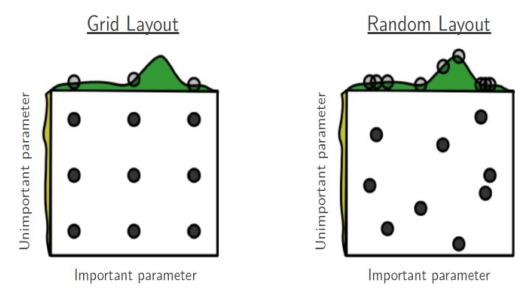
\includegraphics[width=\textwidth,height=3.6cm,keepaspectratio]{images/slide52_grid_random_search.png}
      \end{center}
    \end{column}
  \end{columns}
  \vfill
  {\fontsize{6.5}{8}\selectfont\color{subgray}
    \lr{Bergstra \& Bengio: Random Search for Hyper-Parameter Optimization, JMLR, 2012}
  }
\end{frame}

% Slide 53: Bayesian Optimization
\begin{frame}{بهینه‌سازی بیزی فراپارامترها}{\lr{Bayesian Optimization}}
  \begin{itemize}
    \setlength{\itemsep}{2pt}
    \item \textbf{جستجوی تکاملی} (\lr{Evolutionary Search}): حفظ ترکیباتی از پارامترها که در تکرارهای پیشین کارایی مناسبی داشته‌اند.
    \item \textbf{بهینه‌سازی بیزی} (\lr{Bayesian Optimization}):
    \begin{itemize}
      \setlength{\itemsep}{1pt}
      \item تبدیل تنظیم فراپارامتر به یک مسئله یادگیری ماشین مستقل (پیش‌بینی امتیاز بر اساس پارامترها).
      \item مدل جانشین (\lr{Surrogate Model}) بر پایه فرایندهای گاوسی امتیاز ارزیابی مدل اصلی را پیش‌بینی می‌کند.
      \item هدایت هوشمندانه جستجو به سمت امیدبخش‌ترین نواحی.
    \end{itemize}
  \end{itemize}
  \vspace{2pt}
  \begin{center}
    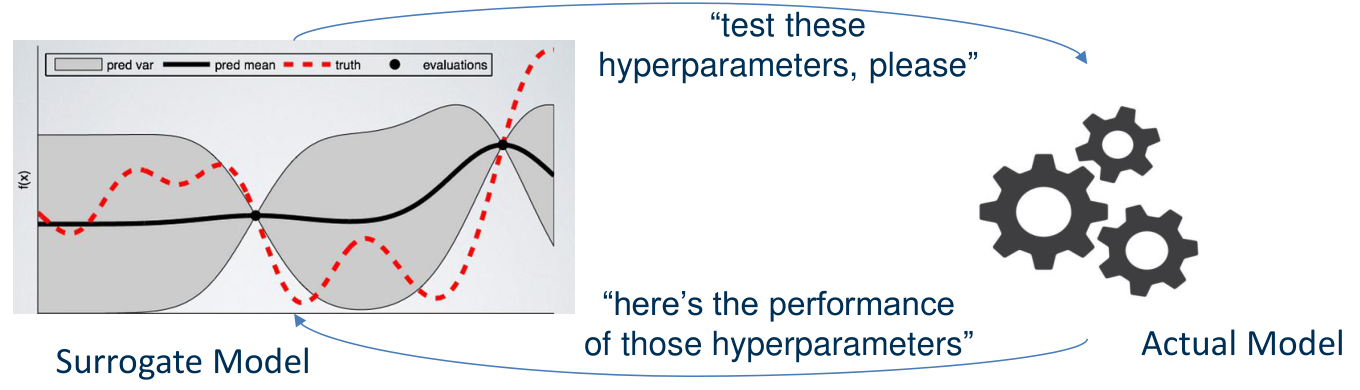
\includegraphics[width=0.92\textwidth,height=3.0cm,keepaspectratio]{images/slide53_bayesian_optimization.png}
  \end{center}
\end{frame}

% Slide 54: The Model Selection Question
\begin{frame}{مسئله انتخاب مدل}{\lr{Model Selection}}
  \begin{itemize}
    \setlength{\itemsep}{12pt}
    \item \textbf{وضعیت فعلی:}
    \begin{itemize}
      \item تعیین کردیم چه ترکیباتی از فراپارامترها باید آزموده شوند.
      \item در عمل اغلب صدها ترکیب فراپارامتر آموزش داده می‌شوند (علت اصلی نیاز به محاسبات ابری).
    \end{itemize}
    \item \textbf{چالش اساسی انتخاب مدل} (\lr{Model Selection}):
    \begin{itemize}
      \item از میان تمام مدل‌های آموزش‌دیده $\mathcal{M}$، چگونه مدل بهینه $m_{\text{best}}$ را انتخاب کنیم که بهترین تعمیم را روی داده‌های نادیده داشته باشد؟
      \item \textbf{پرسش کلیدی:} این ارزیابی و انتخاب مدل روی چه داده‌هایی باید انجام گیرد؟
    \end{itemize}
  \end{itemize}
\end{frame}

% Slide 55: Validation Set
\begin{frame}{انتخاب مدل با مجموعه اعتبارسنجی}{\lr{Model Selection Using a Validation Set}}
  \begin{columns}[T]
    \begin{column}{0.58\textwidth}
      \begin{itemize}
        \setlength{\itemsep}{4pt}
        \item \textbf{اصل تفکیک:} داده‌های انتخاب مدل باید کاملاً از داده‌های آزمون نهایی مجزا باشند، وگرنه مدل به داده آزمون بیش‌برازش می‌شود.
        \item \textbf{گام‌های پنج‌گانه:}
        \begin{enumerate}
          \setlength{\itemsep}{2pt}
          \item تفکیک $D_{\text{train}}$ به داده آموزش $D_{\text{tr}}$ و داده اعتبارسنجی $D_{\text{val}}$.
          \item آموزش مدل‌های $m_i$ روی $D_{\text{tr}}$ با ترکیبات فراپارامتری $p_i$.
          \item انتخاب بهترین پارامتر $p_{\text{best}}$ با آزمون روی $D_{\text{val}}$.
          \item آموزش مدل نهایی $m_{\text{best}}$ روی کل داده‌های $D_{\text{train}}$ با $p_{\text{best}}$.
          \item ارزیابی مدل نهایی $m_{\text{best}}$ روی مجموعه آزمون (\lr{Test Set}).
        \end{enumerate}
      \end{itemize}
    \end{column}
    \begin{column}{0.40\textwidth}
      \begin{center}
        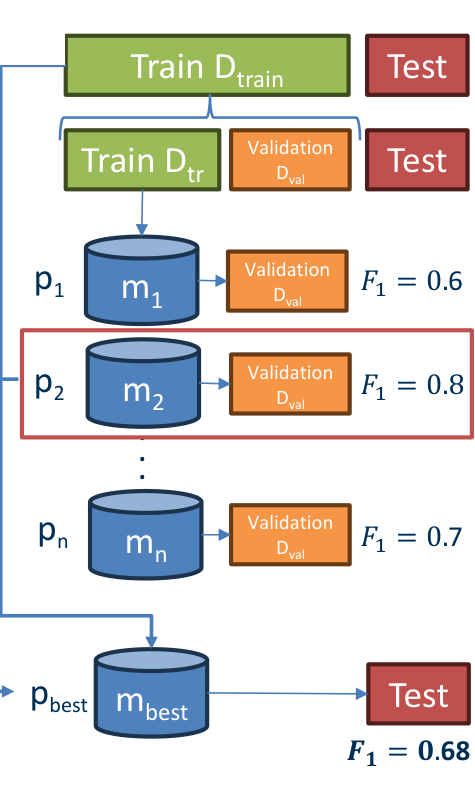
\includegraphics[width=\textwidth,height=4.8cm,keepaspectratio]{images/slide55_val_diagram.png}
      \end{center}
    \end{column}
  \end{columns}
\end{frame}

% Slide 56: Cross-Validation for Model Selection
\begin{frame}{انتخاب مدل با اعتبارسنجی متقاطع}{\lr{Model Selection Using Cross-Validation}}
  \begin{itemize}
    \setlength{\itemsep}{2pt}
    \item اهداف کلیدی در انتخاب مدل:
    \begin{enumerate}
      \item اطمینان از اینکه تمامی نمونه‌ها یک بار برای اعتبارسنجی استفاده شوند.
      \item استفاده حداکثری از داده‌های برچسب‌دار برای آموزش.
    \end{enumerate}
    \item هر دو هدف با استفاده از \textbf{اعتبارسنجی متقاطع برای انتخاب مدل} برآورده می‌شوند:
  \end{itemize}
  \vspace{-0.1cm}
  \begin{center}
    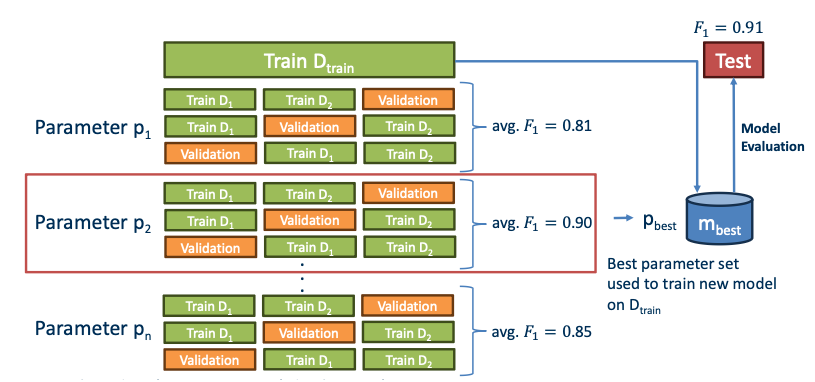
\includegraphics[width=0.92\textwidth,height=4.4cm,keepaspectratio]{images/slide56_cv_model_diagram_clean.png}
  \end{center}
\end{frame}

% Slide 57: Nested Cross-Validation
\begin{frame}{اعتبارسنجی متقاطع تودرتو}{\lr{Nested Cross-Validation}}
  \begin{itemize}
    \item تفکیک دو حلقه متقاطع: حلقه درونی جهت \textbf{انتخاب مدل} و حلقه بیرونی جهت \textbf{ارزیابی تعمیم}.
  \end{itemize}
  \vspace{-0.1cm}
  \begin{center}
    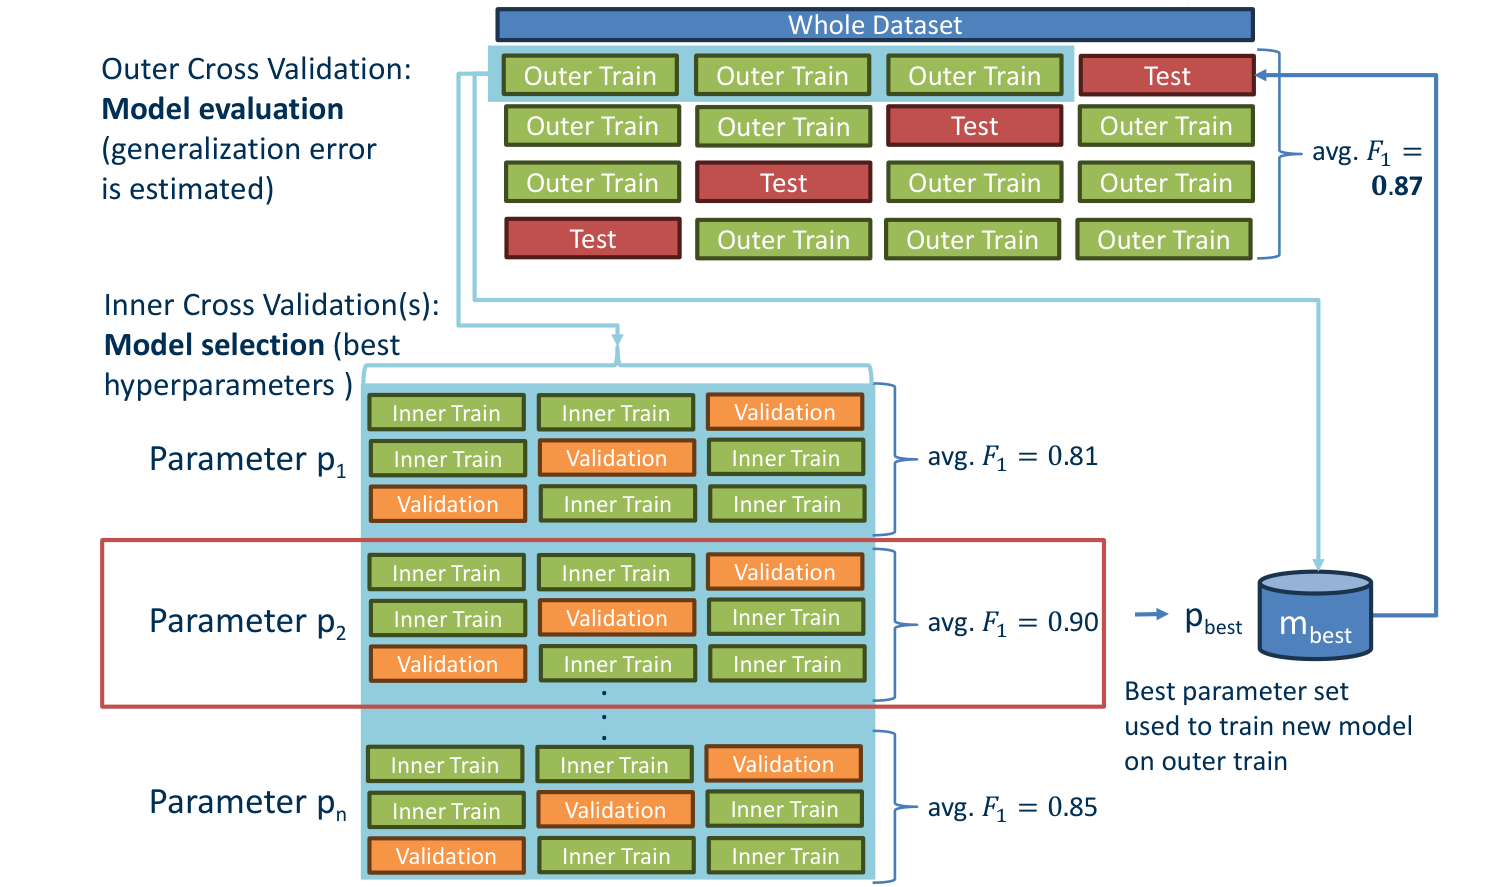
\includegraphics[width=0.95\textwidth,height=4.8cm,keepaspectratio]{images/slide57_nested_cv_diagram.png}
  \end{center}
\end{frame}

% Slide 58: Nested CV in Python
\begin{frame}{اعتبارسنجی متقاطع تودرتو در پایتون}{\lr{Nested Cross-Validation in Scikit-Learn}}
  \begin{itemize}
    \item پیاده‌سازی حرفه‌ای با ترکیب \codeinline{GridSearchCV} و \codeinline{cross\_val\_score} به صورت زیر انجام می‌شود:
  \end{itemize}
  \vspace{0.1cm}
  \begin{latin}
    \begin{minipage}{0.96\textwidth}
      \fcolorbox{codeborder}{codebg}{%
        \begin{minipage}{0.97\textwidth}
          \ttfamily\small
          \textbf{from} sklearn.model\_selection \textbf{import} GridSearchCV, cross\_val\_score\\
          \textbf{from} sklearn.svm \textbf{import} SVC\\[5pt]
          \textcolor{mannheimteal}{\# 1. Define hyperparameter search grid}\\
          parameter\_grid = \{\textcolor{teal}{'C'}: [1, 10, 100, 1000], \textcolor{teal}{'gamma'}: [0.001, 0.01, 0.1, 1]\}\\[4pt]
          \textcolor{mannheimteal}{\# 2. Inner CV: Model selection via GridSearchCV (5 folds)}\\
          estimator\_svm = SVC(kernel=\textcolor{teal}{'rbf'})\\
          estimator\_gs = GridSearchCV(estimator\_svm, parameter\_grid, scoring=\textcolor{teal}{'accuracy'}, cv=5)\\[4pt]
          \textcolor{mannheimteal}{\# 3. Outer CV: Unbiased model evaluation (5 folds)}\\
          accuracy\_cv = cross\_val\_score(estimator\_gs, dataset, labels, cv=5, scoring=\textcolor{teal}{'accuracy'})
        \end{minipage}%
      }
    \end{minipage}
  \end{latin}
\end{frame}

% Slide 59: Overview & Cost Comparison
\begin{frame}{جمع‌بندی رویکردهای انتخاب مدل}{مقایسه هزینه محاسباتی و دقت تخمین}
  \begin{itemize}
    \setlength{\itemsep}{2pt}
    \item \textbf{ارزیابی مدل با اعتبارسنجی یا CV:} از مجموعه آزمون فقط \textbf{یک‌بار} جهت برآورد نهایی خطا استفاده کنید!
    \item هرچه مدل‌های بیشتری آموزش داده شوند، برآورد خطای تعمیم دقیق‌تر و واقع‌بینانه‌تر خواهد بود.
  \end{itemize}

  \begin{center}
    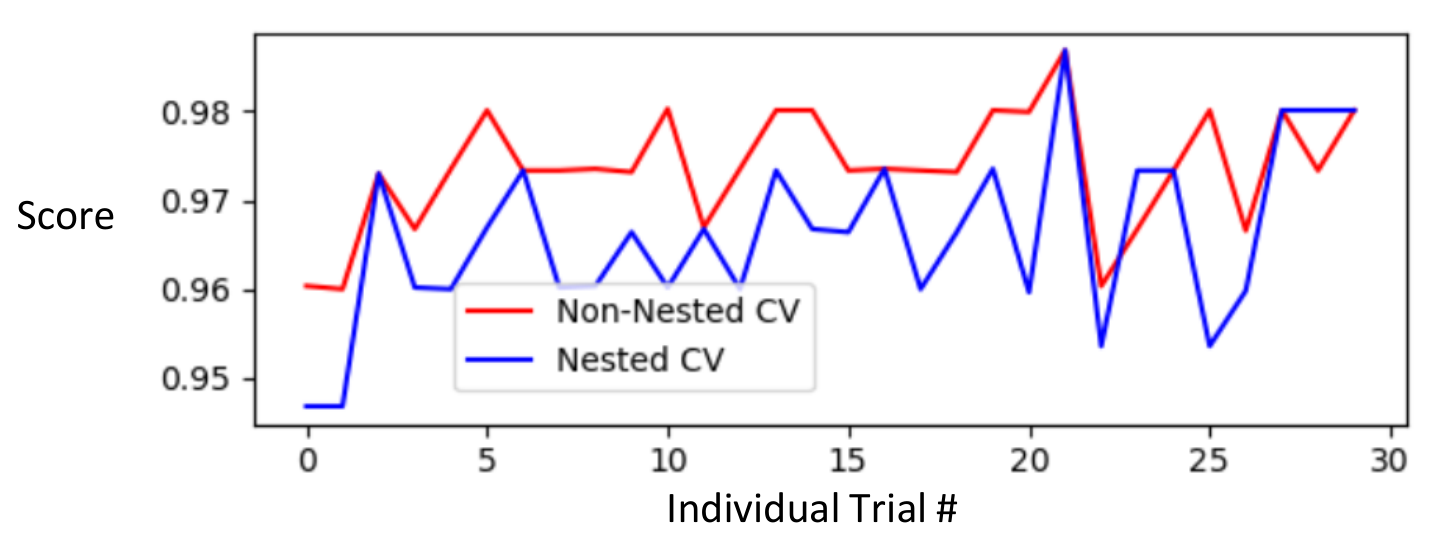
\includegraphics[height=1.95cm,keepaspectratio]{images/slide59_nested_vs_nonnested_plot.png}
  \end{center}

  \begin{itemize}
    \setlength{\itemsep}{2pt}
    \item \textbf{سناریوی مقایسه} (۱۰۰ ترکیب پارامتر با اعتبارسنجی ۵ فولد درونی و بیرونی):
    \begin{itemize}
      \setlength{\itemsep}{2pt}
      \item \textbf{مجموعه اعتبارسنجی:} $|P| + 1 = 100 + 1 = \mathbf{101}$ مدل آموزش‌دیده
      \item \textbf{اعتبارسنجی متقاطع ساده:} $|\text{folds}| \times |P| + 1 = 5 \times 100 + 1 = \mathbf{501}$ مدل آموزش‌دیده
      \item \textbf{اعتبارسنجی تودرتو} (\lr{Nested CV}): $|\text{folds}_{\text{outer}}| \times (|\text{folds}_{\text{inner}}| \times |P| + 1) = 5 \times 501 = \mathbf{2505}$ مدل
    \end{itemize}
  \end{itemize}
\end{frame}

% Slide 60: Feature Selection
\begin{frame}{انتخاب ویژگی}{\lr{Feature Selection}}
  \begin{columns}[T]
    \begin{column}{0.62\textwidth}
      \begin{itemize}
        \setlength{\itemsep}{5pt}
        \item برخی روش‌ها انتخاب ویژگی را به صورت خودکار انجام می‌دهند (مانند درخت تصمیم، جنگل تصادفی و \lr{SVM}).
        \item عملکرد سایر روش‌ها به شدت وابسته به زیرمجموعه ویژگی‌های ورودی است (مانند \lr{k-NN} و بیز ساده).
        \item \textbf{رویکردهای جستجوی خودکار ویژگی:}
        \begin{itemize}
          \item \textbf{انتخاب پس‌رو} (\lr{Backward}): شروع با همه ویژگی‌ها و حذف گام‌به‌گام.
          \item \textbf{انتخاب پیش‌رو} (\lr{Forward}): شروع از بهترین ویژگی منفرد و افزودن متوالی.
        \end{itemize}
        \item استفاده از \textbf{اعتبارسنجی متقاطع تودرتو} جهت تخمین دقیق خطای تعمیم.
      \end{itemize}
    \end{column}
    \begin{column}{0.36\textwidth}
      \begin{center}
        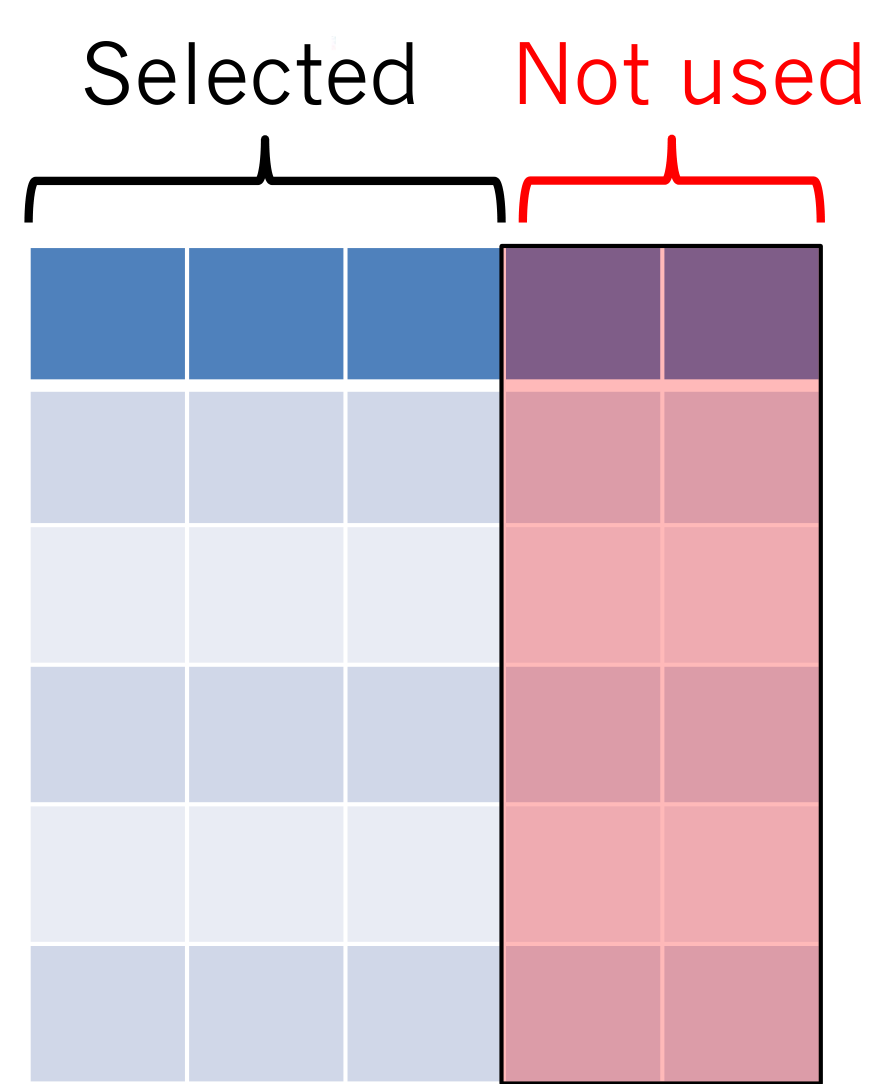
\includegraphics[width=\textwidth,height=4.2cm,keepaspectratio]{images/slide60_feature_selection_diagram.png}
      \end{center}
    \end{column}
  \end{columns}
\end{frame}

% Slide 61: Summary Guidelines
\begin{frame}{دستورالعمل‌های بهینه‌سازی فراپارامتر و انتخاب مدل}{\lr{Best Practices Summary}}
  \begin{itemize}
    \setlength{\itemsep}{7pt}
    \item \textbf{انتخاب فراپارامترها:} همواره بهینه‌سازی فراپارامترها را اجرا کنید؛ در غیر این صورت نمی‌توانید ادعا کنید که یک الگوریتم برای داده‌های شما کارایی ندارد.
    \item \textbf{انتخاب ویژگی:} بررسی کنید که آیا الگوریتم منتخب به انتخاب ویژگی نیاز دارد یا خیر، و در صورت نیاز جستجوی پیش‌رو/پس‌رو انجام دهید.
    \item \textbf{انتخاب مدل:} در حالت استاندارد از \textbf{اعتبارسنجی متقاطع تودرتو} استفاده کنید؛ در صورت کمبود زمان، فضای جستجو را محدود کرده یا از تقسیم تک‌مرحله‌ای (\lr{Train/Val/Test}) استفاده نمایید.
    \item \textbf{نکته طلایی در داده‌های نامتعادل:} فقط داده‌های آموزشی را متوازن (\lr{Balance}) کنید و هرگز توزیع داده‌های آزمون را تغییر ندهید!
  \end{itemize}
\end{frame}
